% !TeX root = article.tex
\section{Numerical examples}

\subsection{Block under tension}
In this section, changes to constraint formulation are clarified by doing few simulation steps
of non constrained, rigid and
elastic-plastic examples using numerical values.

\begin{figure}[htb!]
\centering
\begin{tikzpicture}
\coordinate (O) at (0,0,0);

% axes
\draw[->] (O) -- (1,0,0) node[anchor=north east]{$x$};
\draw[->] (O) -- (0,1,0) node[anchor=north west]{$y$};
\draw[->] (O) -- (0,0,1) node[anchor=south]{$z$};

% 1,3,1 block, base at y=1.5
\draw (1,1.5,0) -- ++(0,3,0) -- ++(-1,0,0);
\draw (0,1.5,1) -- ++(1,0,0) -- ++(0,3,0) -- ++(-1,0,0) -- ++(0,-3,0);
\draw (1,1.5,0) -- ++(0,0,1);
\draw (0,4.5,0) -- ++(0,0,1);
\draw (1,4.5,0) -- ++(0,0,1);

\draw[-Stealth] (0.5,3,0.5) -- ++(0,1.5,0);
\end{tikzpicture}
\caption{Single body model for plasticy processing demonstration.}
\label{fig:tensionModel}
\end{figure}

System has only one dynamic rigid body which is three meters high block of 0.04 \% steel enforced concrete. 
Cross section is one square meter.
Constraint is set so that connecting frame is at top of block. 
In this case frame could be anywhere but if multiple bodies are involved, connecting frame must be defined
so that it reflects scenario under investigation.
Concrete density is $2000 \frac{kg}{m^3}$ and steel density is $7800 \frac{kg}{m^3}$. 
Steel is assumed to handle load in elastic-plastic case. Yield stress of steel is 200 MPa.
Gravity is $10 \frac{m}{s^2}$. Simulation step is $\frac{1}{60} s$ and 10 
iterations are done for single step.
Body is 1.5 meters above rigid ground. In unconstrained case body will hit hit ground at t=0.548 s 
($\sqrt{2 \cdot 1.5 / 10}$).

Single simulation step is done using following substeps. 
In this work, changes are made only to constraint setup and update actions.
\begin{enumerate}
\item Apply gravity to each non static body. 
This step makes programming easier as otherwise each program should add forces due to gravity in each step. 
In this case, $\vec{f}_{ext}$ in  Equation \ref{eq:eomV2} gets added by $\lbrace{0,-60000,0}\rbrace$.
\item Predict unconstrained motion for each body controlled by physics simulation.
Static and kinematic bodies are not processed in this step.
Prediction is done based on current linear and angular velocities of the body.
\item Predict contacts. In this phase, continuous collision detection is done based on simplified objects. 
Each rigid body is represented by sphere geometry and contact prediction is done if body moves more than given threshold value during simulation step. Continuous collision detection is configured for each body. 
Typical scenario that requires continuous collision detection is fast moving bodies that would otherwise go through walls.
\item Perform discrete collision detection. All overlapping bodies are processed and manifoldPoints are created for
each detected contact at end of simulation step. 
In unconstrained case, contact is detected after $t$=0.55 s if continuous collision detection is not used and manifolds distance gets negative value (-0.058 m).
\item Calculate simulation islands(groups). Bodies that are near each other based on contact prediction or discrete collision detection
 or connected with constraints are grouped in same group.
\item Solve constraints. Both contact and other constraints are processed in this step. 
 This step is subdivided to setup, iterations and finish phases. 
In setup phase constraints are queried for positional errors for calculation of $c$ in
Equation \ref{eq:constraintEquation} and maximum and minimum impulses in Equations \ref{eq:lambdaLow} and 
\ref{eq:lambdaHigh}.
In finish phase constraint forces are calculated if requested and velocities of bodies are updated.
\item Integrate transforms using velocities modified in previous step.
\item Update actions (callbacks) are called. 
In elastic-plastic case, plasticity is summed and equilibrium point of elastic part is updated if maximum force or moment is exceeded.
\item Activation state of bodies is updated. 
To avoid extra calculation bodies are as default put to sleeping state if linear and angular velocities of body are less than
given threshold values (default 0.8 and 1.0) longer than set time limit (2.0).
\end{enumerate} 

Equation \ref{eq:constraintEquation} is simplified
to \ref{eq:fixedConstraint} in constrained cases.
\begin{itemize}
\item No rotation takes place. $\omega_1$ and $\omega_2$ are zeros.
\item Constraint force mixing can be ignored.
\item Only vertical velocity is handled.
\item Other involved body is rigid and it does not move.
\end{itemize} 

\begin{equation} \label{eq:fixedConstraint}
m v_y = c 
\end{equation}

Equations \ref{eq:lambdaLow} and \ref{eq:lambdaHigh} are not active for fixed case.
For elastic-plastic case maximum impulse is set to product of yield stress, area of steel enforcement and time step (1330).

Method btSequentialImpulseConstraintSolver::solveGroupCacheFriendlySetup
in \bullet\ was used to pick up values for internal variables described in Figure \ref{fig:solVars}. 

\begin{figure}[htb!]
\begin{description}
\item[velError] is calculated using velocities and external impulses of connected bodies.  
 \begin{description}
\item[In constraint cases,] main contibutor is bodies relative speed at joint point.
\item[In contact case,] main contributor is bodies relative speed at point of contact. 
Bodies are not allowed to penetrate each other. Restitution increases velError.
If contact is not penetrating velError is reduced by $penetration * timeStep$.
\end{description}
\item[posError] is calculated by constraint. It is significant factor in designing stable constraints.
 \begin{description}
 \item[In fixed case,] value is about 12 times actual position error. Factor 12 is based on time step (60) 
 and default value of error reduction parameter (erp) which has value of 0.2 in this context.
 \item[In elastic plastic case,]  value is set to zero if impulse would be larger than maximum impulse or
spring simulation cannot be done in stable way.
 \item[In contact case,] value is zero if there is no penetration. For penetration cases it is 
$\frac{-penetration\, erp}{timeStep}$. In contact cases default value for erp is 0.8.
 \end{description}
\item[rhs (c)] is calculated by velError jInv + posError jInv
\item[jInv] is calculated using masses and inertias of connected bodies and constraint geometry. 
 \begin{description}
\item[In constraint cases,] it is mass of body (6000).
\item[In contact case,] it varies below mass of body.
\end{description}
\item[Impulse] is impulse applied to body during timestep.
 \begin{description}
\item[In constraint cases,] it is obtained from btJointFeedback structure.
\item[In contact case,] it is obtained by summing applied impulses from active manifolds.
\end{description}
\item[erp] Error reduction parameter (0...1) is used to handle numerical issues e.q. object drifting. 
Setting erp to 1 would in theory eliminate error in one step but in practice value of 0.2 - 0.8 is used in most cases.
\end{description}
\caption{Internal variables used in \bullet\ in constraint solving.}
\label{fig:solVars}
\end{figure}

Actual values for unconstrained case without continuous collision detection
are shown in table \ref{tab:freeBlockValues}. Penetration is detected at time 0.567 s when
{\it velError} is 5.67 (5.5+0.167) and
{\it posError} is 2.8 (0.058*0.8/0.0167). Impulse is 34000 and contact force is thus about 2 MN (34000/0.0167).
After few steps location and position stabilize although internally calculation is needed for each time step
until body is deactivated.

\begin {table}[htb!]
\begin{center}
\begin{tabular}{|l| l|l| l|l|l|l|l|}
\hline
{\bf Time} & 
{\bf Location} &
{\it velError} & {\it penetration} & {\it posError} & {\it rhs} &
{\bf Velocity} & 
{\bf Impulse} \\  \hline
0.017 &  0 & & & &  &-0.17 & 0 \\  \hline
0.550 &  -1.558 & & & & & -5.5 & 0 \\  \hline
0.567 &  -1.511 & 5.67 &-0.058 &2.8 &  21270 & 0.01 & 34000 \\  \hline
0.583 &  -1.502 & 0.14 &-0.011 & 0.54& 2570  & 0.55 & 420 \\  \hline
0.600 &  -1.496 & -0.38&-0.002 & 0.1  & -1000& 0.38 & 0 \\  \hline
0.617 &  -1.492 &-0.44 & 0.004 & 0     & -1600& 0.22 & 0 \\  \hline
0.717 &  -1.497 &0.004-0.08  &-0.0003-0.001 &0-0.01 & 10-400 & -0.01 & 400 \\  \hline
0.817 &  -1.499 & & & & & -0.08 & 700 \\  \hline
0.917 &  -1.500 & & & & & -0.001 & 1000 \\  \hline
\end {tabular}
\end{center}
\caption {Simulation values for unconstrained case. 
For internal contact values typical values are shown
as number of contacts and values at contact points are different.} 
\label{tab:freeBlockValues} 
\end {table}

Actual values for unconstrained case with continuous collision detection (ccd) using 1.5 
as radius of ccd sphere and 0.001 as ccd motion threshold
are shown in \ref{tab:freeBlockValuesWithCcd}. Collision is detected at time 0.550 s when
{\it velError} is  3.5 (5.34+0.167)-0.033/0.0167 and
{\it posError} is  0 as collision is detected before penetration. 
It should be noted that in general ccd sphere should not extend actual body as 
premature contacts are created if collision takes place in those regions.

\begin {table}[htb!]
\begin{center}
\begin{tabular}{|l| l|l| l|l|l|l|l|}
\hline
{\bf Time} & 
{\bf Location} &
{\it velError} & {\it penetration} & {\it posError} & {\it rhs} &
{\bf Velocity} & 
{\bf Impulse} \\  \hline
0.017 &  0 & & & &  &-0.17 & 0 \\  \hline
0.550 &  -1.500 & 3.5 & 0.033 & 0 & 21000& -2 & 21000 \\  \hline
0.567 &  -1.500 & 2.17 & 0 & 0  &  8100 & 0.01 & 13000 \\  \hline
0.583 &  -1.500 & 0.15 & 0 & 0 & 600  & 0 & 937 \\  \hline
0.600 &  -1.500 & 0.17 & 0 & 0 & 600  & 0 & 1040 \\  \hline
\end {tabular}
\end{center}
\caption {Simulation values for unconstrained case with continuous collision detection. } 
\label{tab:freeBlockValuesWithCcd} 
\end {table}

Values for fixed constraint are shown in table
\ref{tab:fixedBlockValues}. Constraint is activated in second step and positional error is corrected
about 20 \% in each step as requested by using erp value 0.2.

\begin {table}[htb!]
\begin{center}
\begin{tabular}{|l|l| l| l|l|l|l|}
\hline
{\bf Time} & 
{\bf Location} &
{\it velError} & {\it posError} & {\it rhs} &
{\bf Velocity} & 
{\bf Impulse} \\  \hline
0.017 & -0.0028 &  & & & -0.17 & 0 \\  \hline
0.033 & -0.0022 & 0.33 & -0.033 & -2200 & 0.033 & 2200 \\  \hline
0.050 & -0.0018 & -0.13 & -0.027 & -960 & 0.027 & 960 \\  \hline
0.067 & -0.0014 &-0.14 & -0.021 & -970 & 0.021 & 970 \\  \hline
0.35... & 0 &-0.17 & $\approx$ 0 & -1000 &0.0 & 1000 \\  \hline
\end {tabular}
\end{center}
\caption {Constraint parameter values for fixed constraint} \label{tab:fixedBlockValues} 
\end {table}

There are currently two alternative six-dof-spring constraint implementations in \bullet\ and 
in this work elastic-plastic versions of both of them are developed. 

Table  \ref{tab:ep2Parameters} summarizes most significant parameters for this study.
There are also e.g. parameters for controlling joint motors.
Additional equation is created for each additional constraint. 
Enabled springs and motors add one row and
limits add one if upper and lower are same and two if both upper and lower limits are defined.

\begin {table}[htb!]
\begin{center}
\begin{tabular}{|l|p{10cm}|}
\hline
{\bf Parameter} & 
{\bf Description} 
\\ \hline
lowerLimit &  
minimum allowed translation or rotation
 \\  \hline
upperLimit &  
maximum allowed translation or rotation
 \\  \hline
springStiffness & elastic spring stiffness
 \\  \hline
enableSpring & defines if spring is active
 \\  \hline
springStiffnessLimited & should elastic behaviour be tuned to avoid instability
 \\  \hline
equilibriumPoint & should elastic behaviour be tuned to avoid instability
 \\  \hline
currentLimit & describes state of constraint \newline
 0: not limited \newline
 3: loLimit=hiLimit \newline 
 4: current value is between loLimit and HiLimit
 \\ \hline

\end {tabular}
\end{center}
\caption {Selected constraint parameters for elastic-plastic constraint 2} \label{tab:ep2Parameters} 
\end {table}


Values for elastic-plastic case are shown in tables \ref{tab:epBlockValues}.
Body drops freely during first simulation step and 
gains enough kinetic energy so that higher impulses are needed in few following steps.
This causes plastic strain during next three steps.

\begin {table}[htb!]
\begin{center}
\begin{tabular}{|l|l| l| l|l|l|l|l|}
\hline
{\bf Time} & 
{\bf Location} &
{\it velError} & {\it posError} & {\it rhs} &
{\it velocity} & 
{\bf Impulse} & 
{\bf Plastic strain} \\  \hline
0.017 & -0.0028 &-0.17 & 0 & -1000 & -0.17 & 0 & 0 \\  \hline
0.033 & -0.0046 &-0.33 & 0 & -2000 & -0.11 &  1330 & 0.001 \\  \hline
0.050 & -0.0056 &-0.28 & 0 & -1670 & -0.056 &  1330 & 0.003 \\  \hline
0.067 & -0.0056 &-0.22 & 0 & -1340 &  -0.001&  1330 & 0.004\\  \hline
0.083... & -0.0056  & -0.17 & 0 & -1000 &  0.0&  1000 & 0.004\\  \hline
\end {tabular}
\end{center}
\caption {Constraint parameter values for elastic-plastic constraint} \label{tab:epBlockValues} 
\end {table}

Six-dof-spring constraint 2 has optional feature to avoid unstability by automatically softening constraint
spring. Feature is activated if current timeStep is too large for spring-mass system simulation.
The feature is trigged based on the equation below 
\begin{equation} \label{eq:frequencyLimited}
\sqrt{ k /  m_{min}} dt > 0.25 
\end{equation}
where $k$ is elastic spring stiffness between bodies,
$m_{min}$ is smaller of connected masses or inertias and $dt$ is integration timestep.

If this feature is active for elastic-plastic constraint 2 constraint  
it does not report positional error but it allows full plastic capacity to be used for correcting
velocity based error instead of force provided by spring.
In this scenario object behaves as depicted in table \ref{tab:ep2BlockValues} i.e. it does not move at all.

\begin {table}[htb!]
\begin{center}
\begin{tabular}{|l|l| l| l|l|l|l|l|}
\hline
{\bf Time} & 
{\bf Location} &
{\it velError} & {\it posError} & {\it rhs} &
{\bf Velocity} & 
{\bf Impulse} & 
{\bf Plastic strain} \\  \hline
0.017... &  0 & -0.17  & 0 & -1000 & 0       & 1000 & 0 \\  \hline
\end {tabular}
\end{center}
\caption {Constraint parameter values for elastic-plastic constraint 2} \label{tab:ep2BlockValues} 
\end {table}

\subsection{Charpy impact test}
Simulation of Charpy impact test was used to benchmark approach in more complicated scenario. 
Material is steel. Density is 7800 $\frac{kg}{m^{3}}$. Young’s modulus is 200 GPa.
Specimen dimensions are 10x10x55 mm with 2 mm notch in middle which is taken into account in calculations.
Support anvils initially have 40 mm open space between them. Their width is 40 mm. 
Hammer is 0.5 m wide and 0.25 m high, thickness is 0.02 m. Mass is 19.5 kg.
Hammer has 40 mm draft.
If specimen bends about 1.9 radians (108 degrees) it will go between anvils.
Expected energy loss is product of plastic moment of section, hinge angle needed for specimen to go through supports and 
yield stress of specimen. For hinge angle of 1.9 radians and yield stress of 400 MPa expected energy 
loss is 122 J.

Usually \bullet\ simulations are done using fixed time step of 1/60 s i.e. 16.67 ms. 
For this case that is too large. 
Default time step was selected to be 5 ms outside impact time and 0.1 ms during impact. 
Automatic time stepping routine changes timestep so that at angles higher than 0.2 5 ms time step is
used and adjusts it linearly to selected time step between angles of 0.2 and 0.05.

Table \ref{tab:ep2ts} shows energy loss for few timesteps as example to demonstrate sensitivity of solution
using  elastic-plastic constraint 2.

\begin {table}[htb!]
\begin{center}
\begin{tabular}{| c| c|l|}
\hline
{\bf Timestep[ms]} & {\bf Energy loss [J]} & {\bf Notes} \\ \hline
 0.2 &  170 & specimen penetrates hammer  \\ \hline
 0.1 &  120 & \\ \hline
 0.05 &  150 & \\ \hline
\end {tabular}
\end{center}
\caption {Energy loss for few timesteps} \label{tab:ep2ts} 
\end {table}

Figure \ref{fig:charpy} shows screenshot from simulation.
\begin{figure}[htb!]
\centering
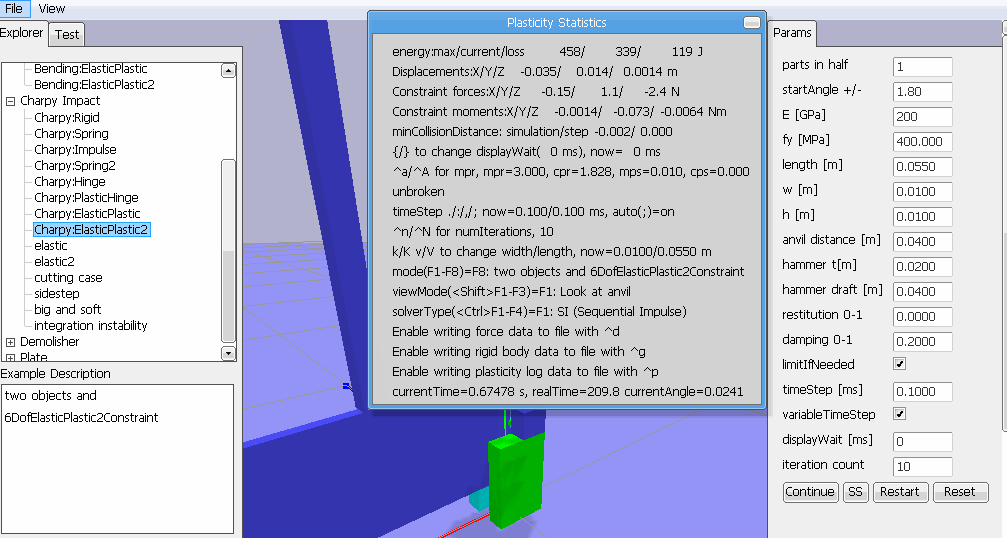
\includegraphics[height=8cm]{figs/article-charpy}
\caption{Simulation of Charpy impact test}
\label{fig:charpy}
\end{figure}


\subsection{Demolisher}
Demolisher is  collection of possible scenarios that can be added to games to provide ductile joints between
rigid bodies.  Simulation can be done in real time on modest hardware. 
Figure \ref{fig:demolisher} shows three screenshots from simulation.

\begin{figure}[htb!]
\centering
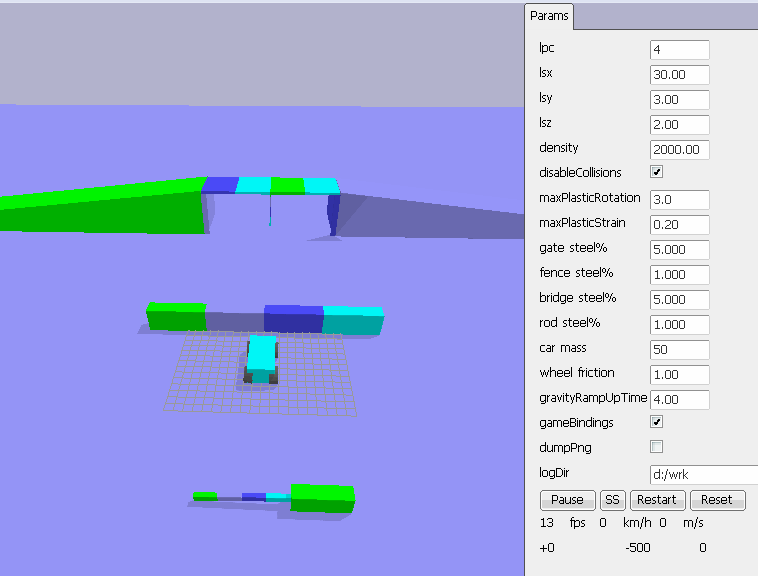
\includegraphics[height=5cm]{figs/demolisher-pre}
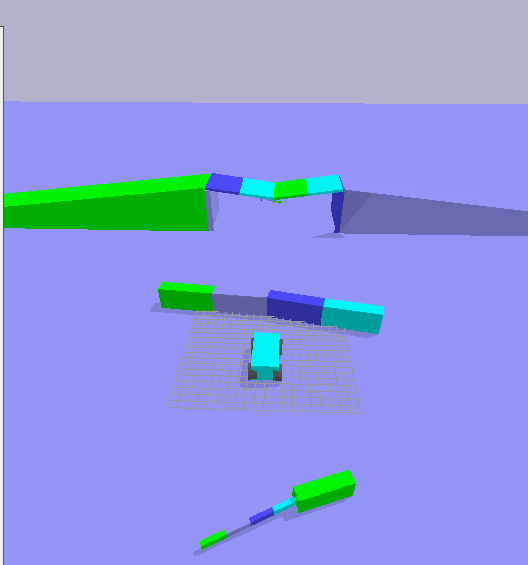
\includegraphics[height=5cm]{figs/demolisher-wip}
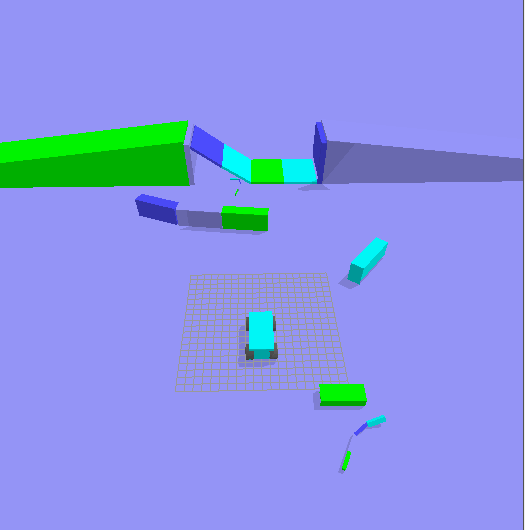
\includegraphics[height=5cm]{figs/demolisher-done}
\caption{Simulation of Demolisher scenario}
\label{fig:demolisher}
\end{figure}

Vehicle is modelled as single box btRaycastVehicle with four driving wheels. Wheels are rendered for visual feedback.
In left picture, initial state is shown. Gate in front is modelled to be so slender that it has visible elastic deflection.
Gate support is modelled as heavy box.
Bridge has rigid ramps and supports at both ends.
Gravity is applied gradually to avoid collapse of bridge at start of simulation.
In middle picture,  bridge is shown in state where car has driven once over bridge without stopping and
other bodies have taken light damage.
In right picture, some of joints have been broken.

